\chapter{\label{sec:filippov}Filippov rendszerek}

%\todo[inline]{CsB: Formázás, azt hiszem kész azt az egy ábrát kivéve}

Tekintsük a
%
\begin{equation}
%\[
\dot{x}=\left\{
\begin{matrix}
F_1(x), \, \mathrm{ha} & H(x) > 0\\
F_2(x), \, \mathrm{ha} & H(x) < 0
\end{matrix}
\right.
%\]
\end{equation}
%
\noindent dinamikai rendszert. Feltesszük, hogy 
$\left.F_1\right|_{H(x)=0} \neq \left.F_2\right|_{H(x)=0}$,
azaz a két vektormező különböző szögben éri el a 
%
\begin{equation}
\sum=\{x:H(x)=0\}
\end{equation}
%
\noindent úgynevezett, \emph{kapcsolófelületet}  (\textit{discontinuity surface} vagy \textit{switching manifold}). Kapcsolófelületre mutat példát a \ref{fig:kapcsolofelulet}.~ábrán látható fekete szaggatott vonal.

\begin{figure}[!h]
\centering
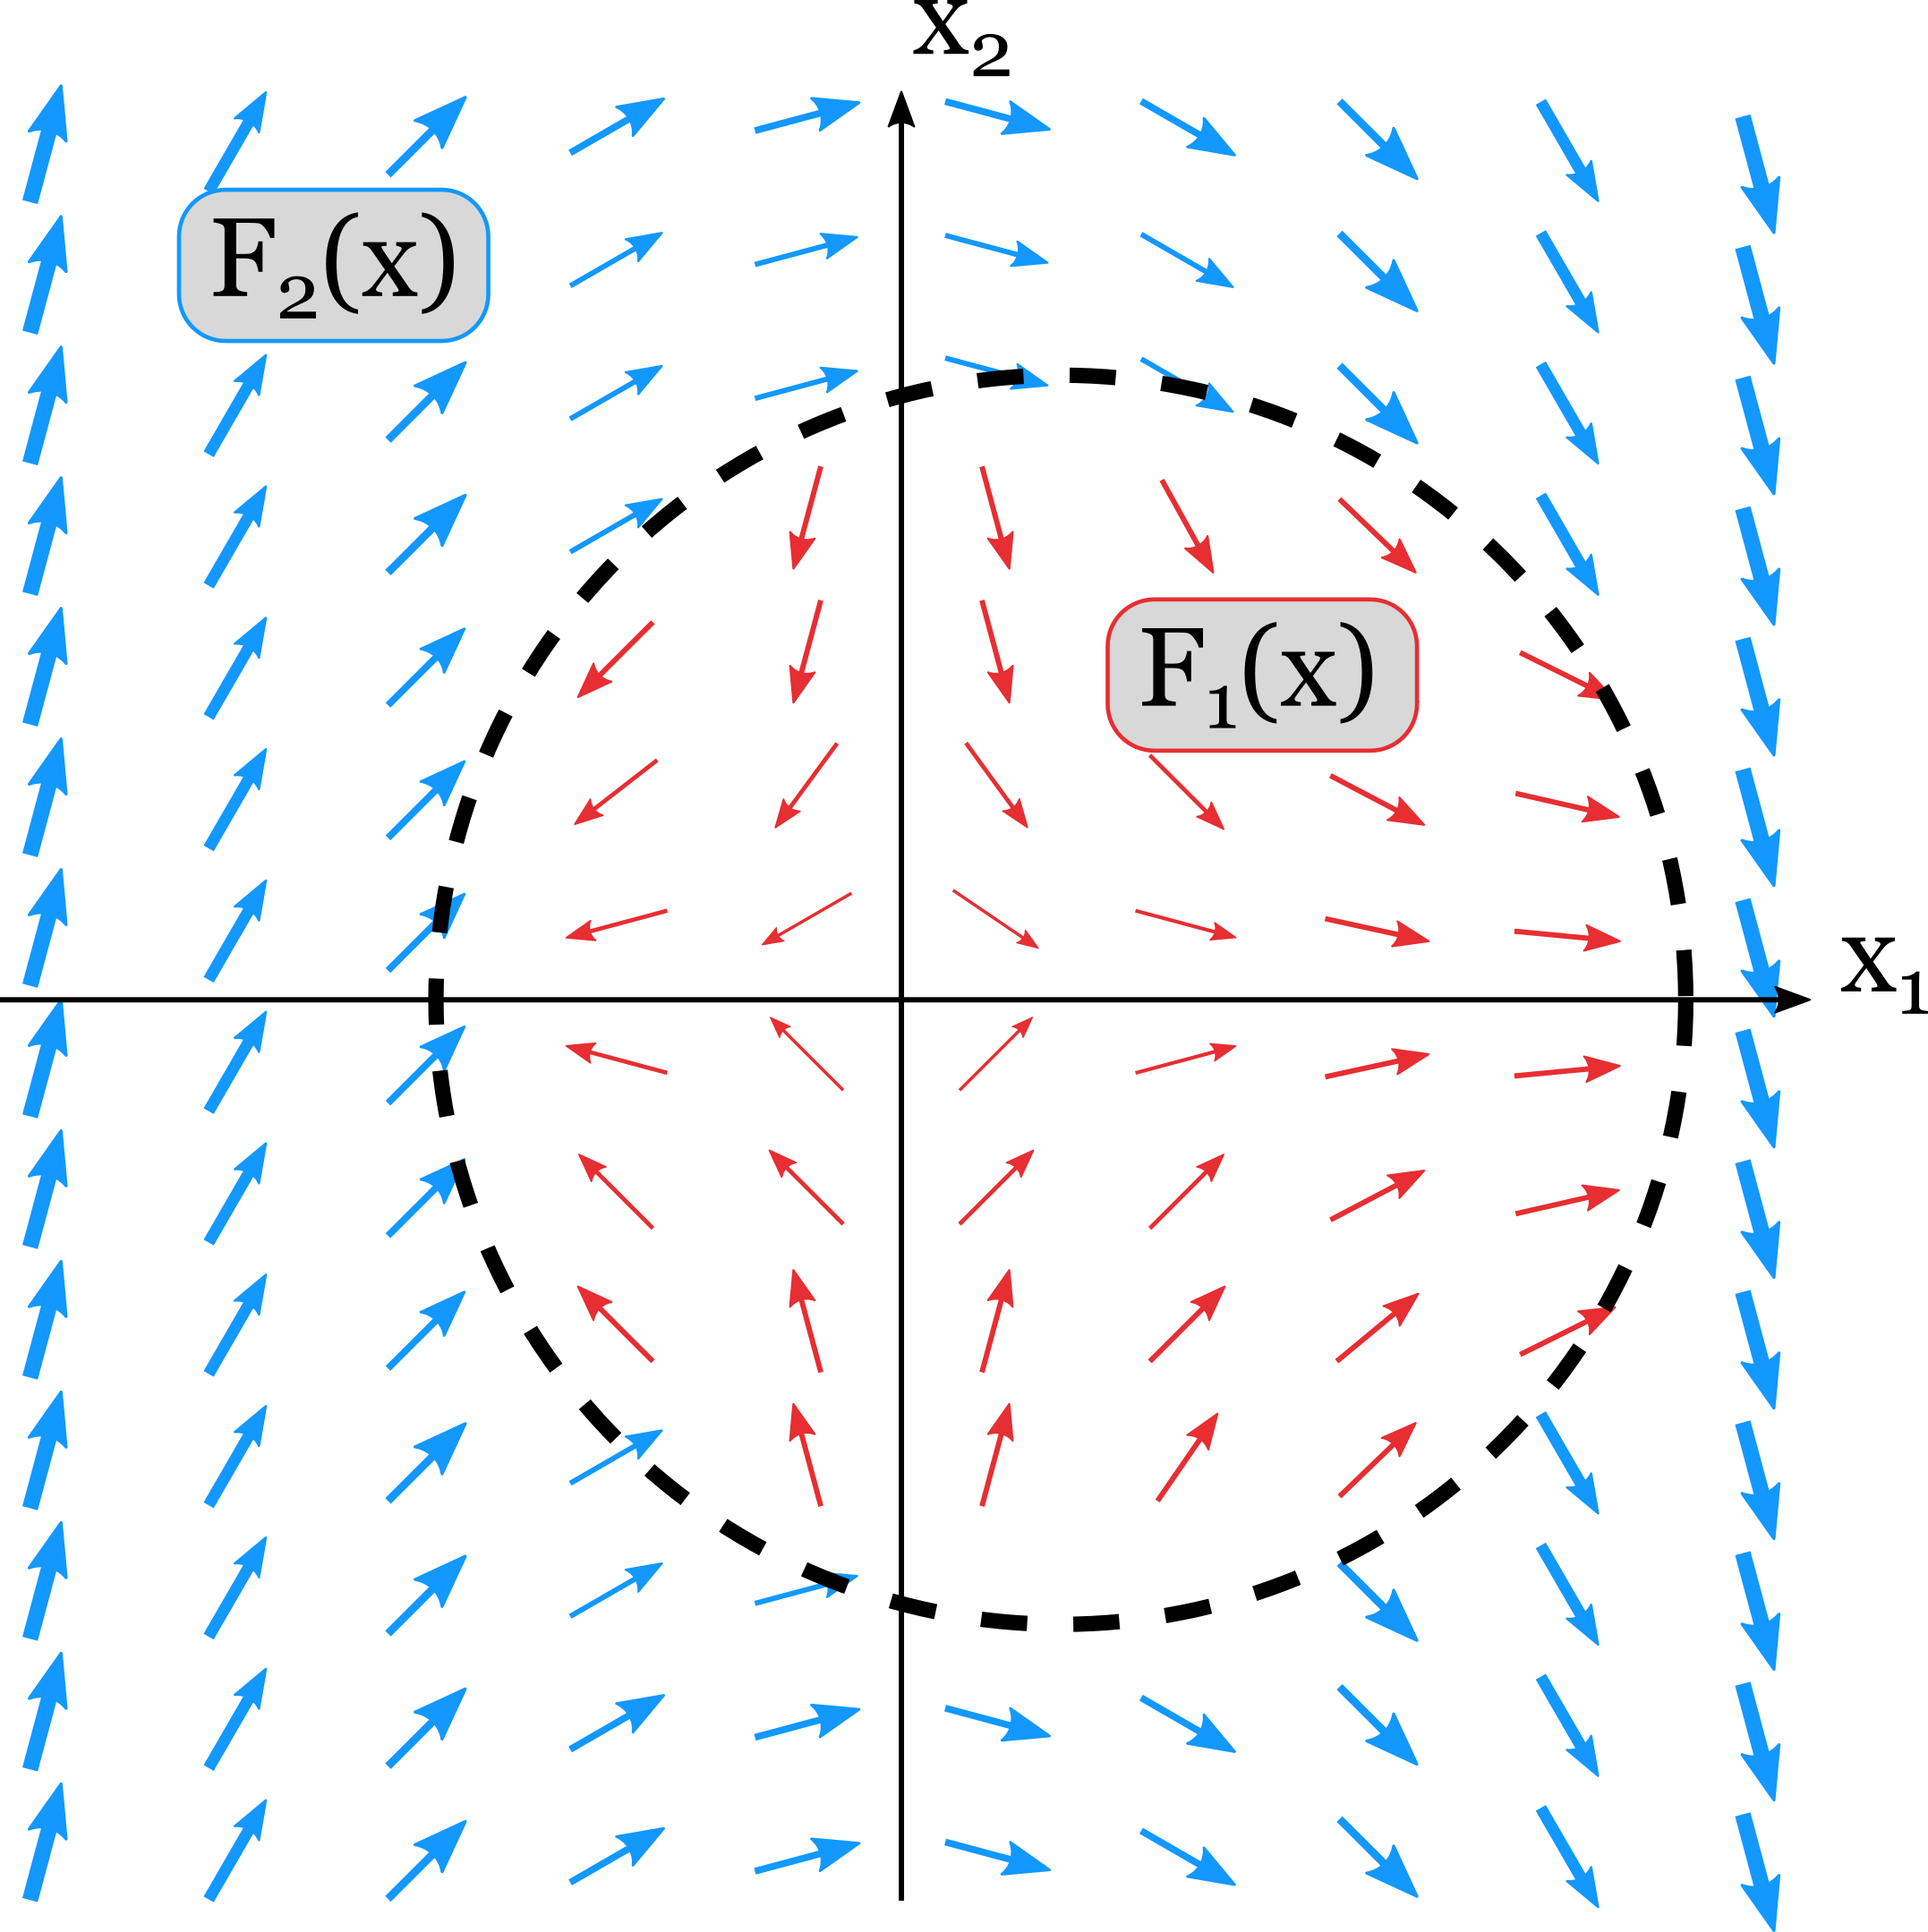
\includegraphics[width=0.5 \textwidth]{graphics/discontinuity_surface_fancy.png}
\caption{Példa kapcsolófelületre (jelen esetben egy kör), amely elválasztja a két dinamikát egymástól.}
\label{fig:kapcsolofelulet}
\end{figure}

Továbbá bevezetjük
%
\begin{equation}
H_x=\nabla H=\begin{pmatrix}
\frac{\partial H}{\partial x_1}&\frac{\partial H}{\partial x_2} &\dots 
\end{pmatrix}^{\rm T}
\end{equation}
%
\noindent \emph{gradienst}, amely $F_1$ növekedésének irányába mutat és merőleges a felületre.
 
\emph{Csúszófelületnek} (sliding region) nevezzük a $\sum$ kapcsolófelület azon rész-
halmazát, melyre $\langle F_1, H_x \rangle<0$ és $\langle F_2, H_x \rangle> 0$ skalárszorzat teljesül. Ezen felületet $\sum_s$-ként jelöljük, ahol $s$ index a $sliding$-ra utal. A csúszófelületen a két dinamikai rendszerhez tartozó trajektóriák csúszófelületre merőleges komponensei egymás felé, azaz befelé mutatnak. Csúszófelületre mutat példát a \ref{fig:csuszofelulet}.~ábra.

\begin{figure}[!h]
\centering
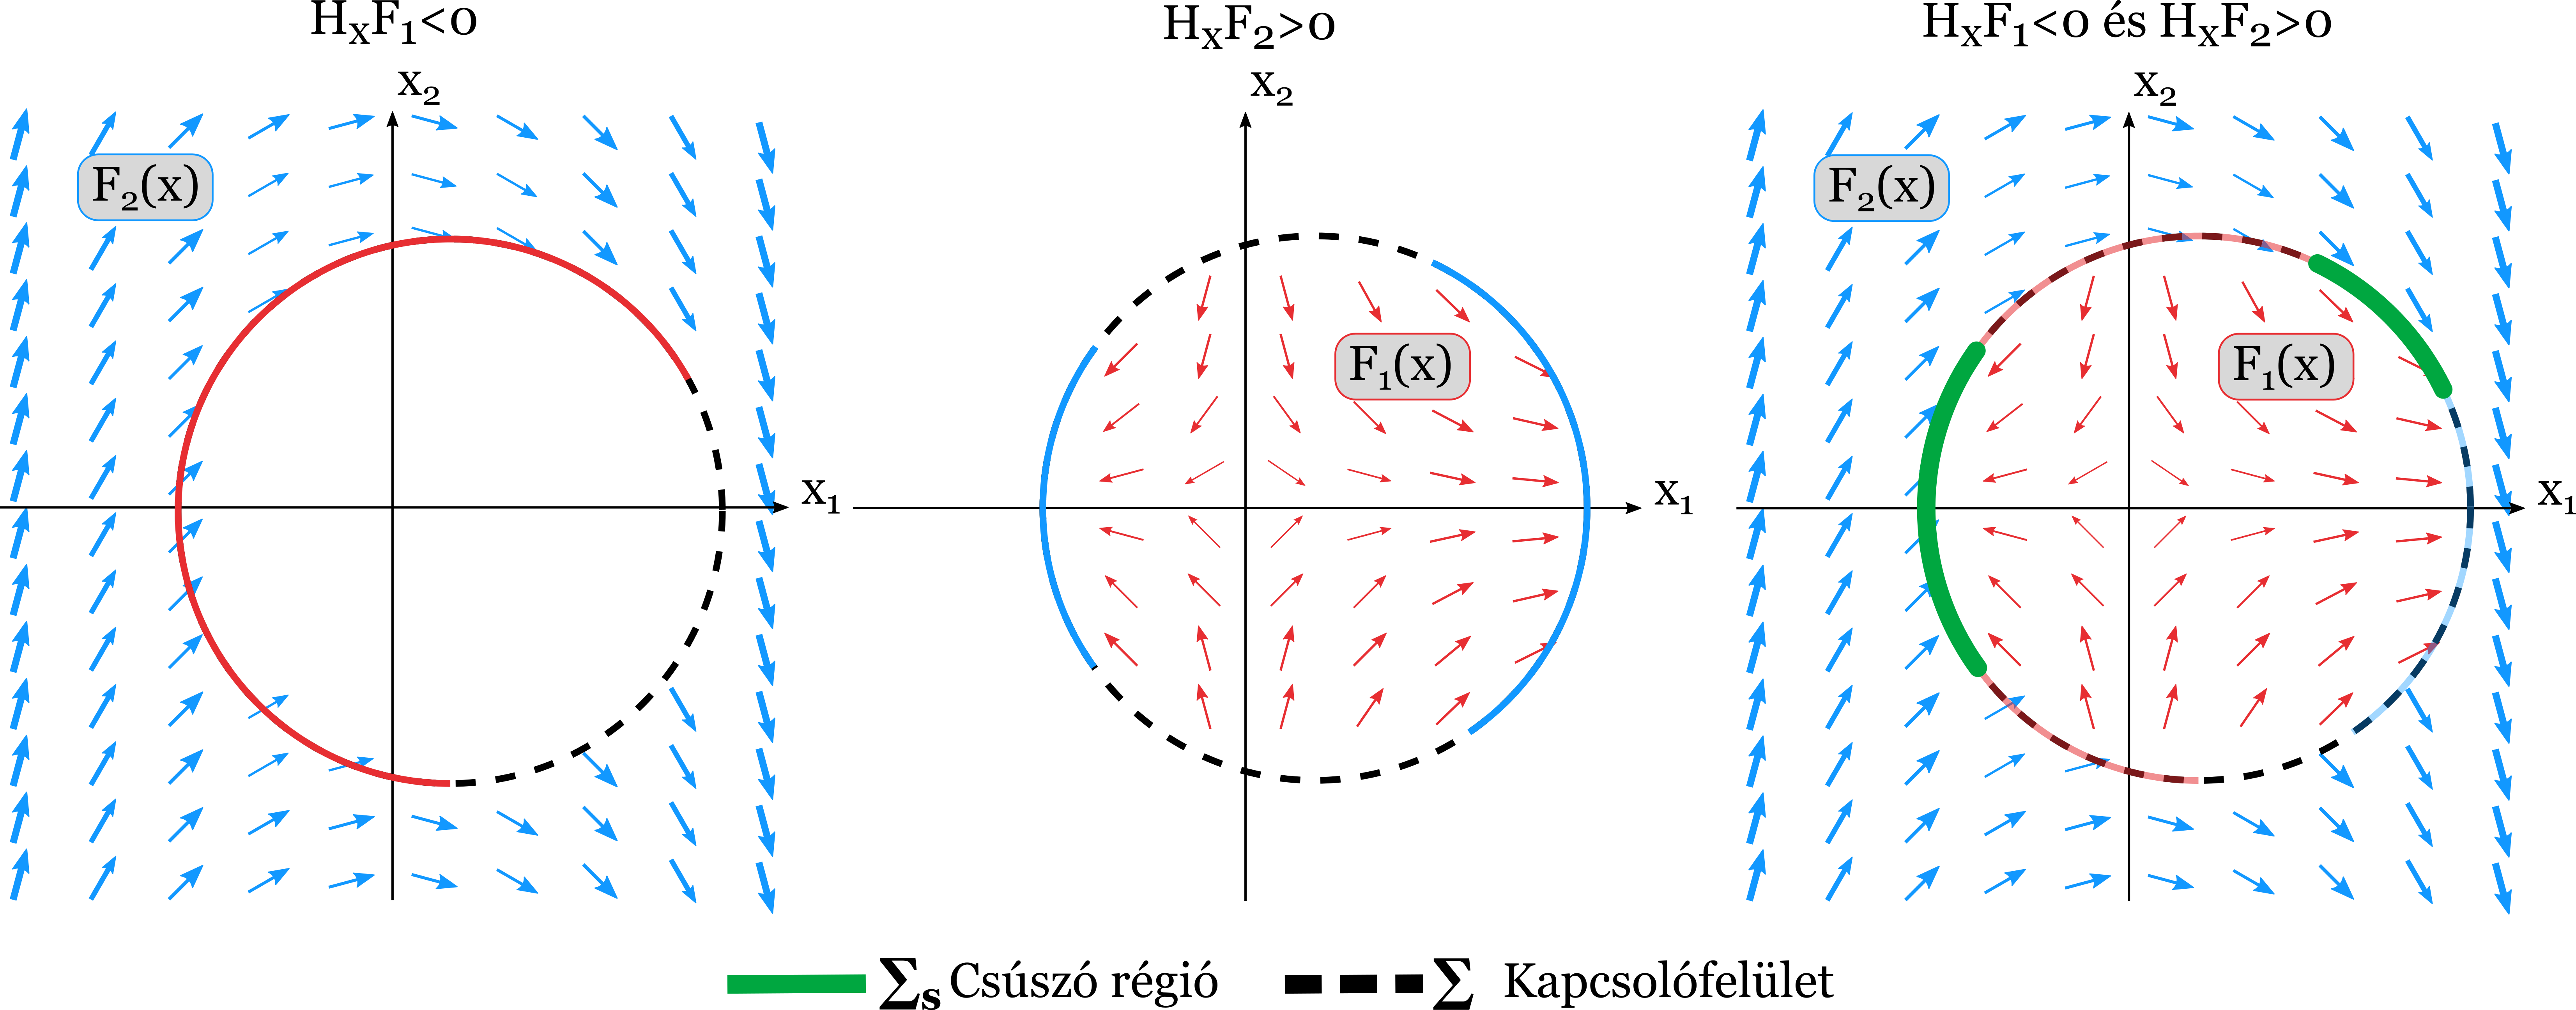
\includegraphics[width=\textwidth]{graphics/sliding_region_fancy.png}
\caption{Példa csúszófelületre.}
\label{fig:csuszofelulet}
\end{figure}

A csúszófelületen uralkodó dinamikát az
%
\begin{equation}
F_s=F_1(1-\alpha)+F_2\alpha 
\end{equation}
%
\noindent egyenlet írja le. Vagyis lineárisan interpolálunk a két vektormező között oly módon, hogy $\alpha$-t úgy adjuk meg, hogy $F_s\perp H_x$ teljesüljön. Ez akkor lesz igaz, ha $F_s$ és $H_x$ skaláris szorzata zérus:
%
\begin{equation}
\langle F_s, H_x \rangle =0 \,,
\end{equation}
%
\noindent tehát
%
\begin{equation}
\langle F_s, H_x \rangle = \langle F_1, H_x \rangle (1-\alpha) + \langle F_2, H_x \rangle \alpha = 0\,,
\end{equation}
%
\noindent melyből kifejezhető $\alpha$ értéke a következőképpen:
%
\begin{equation}
\alpha=\frac{\langle F_1, H_x \rangle}{\langle F_1-F_2, H_x \rangle}\,. 
\end{equation}
%
Jellemzően a $\sum _s$ csúszófelületen a dinamika nagyon egyszerű és exponenciálisan tart(hat) az egyensúlyi helyzet felé (ha van ilyen). Ezt hívjuk \emph{csúszómód szabályozásnak} (\textit{sliding mode control}).

\section{Példa: Munkahenger pozíciójának csúszómód szabályozása}

Tekintsük a \ref{fig:munkahenger}.~ábrán látható elrendezést, mely munkahenger pozíciójának csúszómód szabályozására mutat példát. A hidraulikus tápegység (nyomásforrás) valamekkora $\Delta \tilde{p}>0$ konstans nyomást tud kiadni. A hengervezérlő szelep állásától függően a hidraulikus munkahengerbe $+\Delta \tilde{p}$ vagy $-\Delta \tilde{p}$ nyomás kerül. Ennek hatására a hengerfej jobbra vagy balra mozdul el. Célunk, hogy a munkahengert $x_{\rm k}$ kívánt pozícióba juttassuk a munkahenger csúszómód szabályozása által. Ehhez rendelkezésünkre áll egy PD szabályozó.

\begin{figure}[!h]
\centering
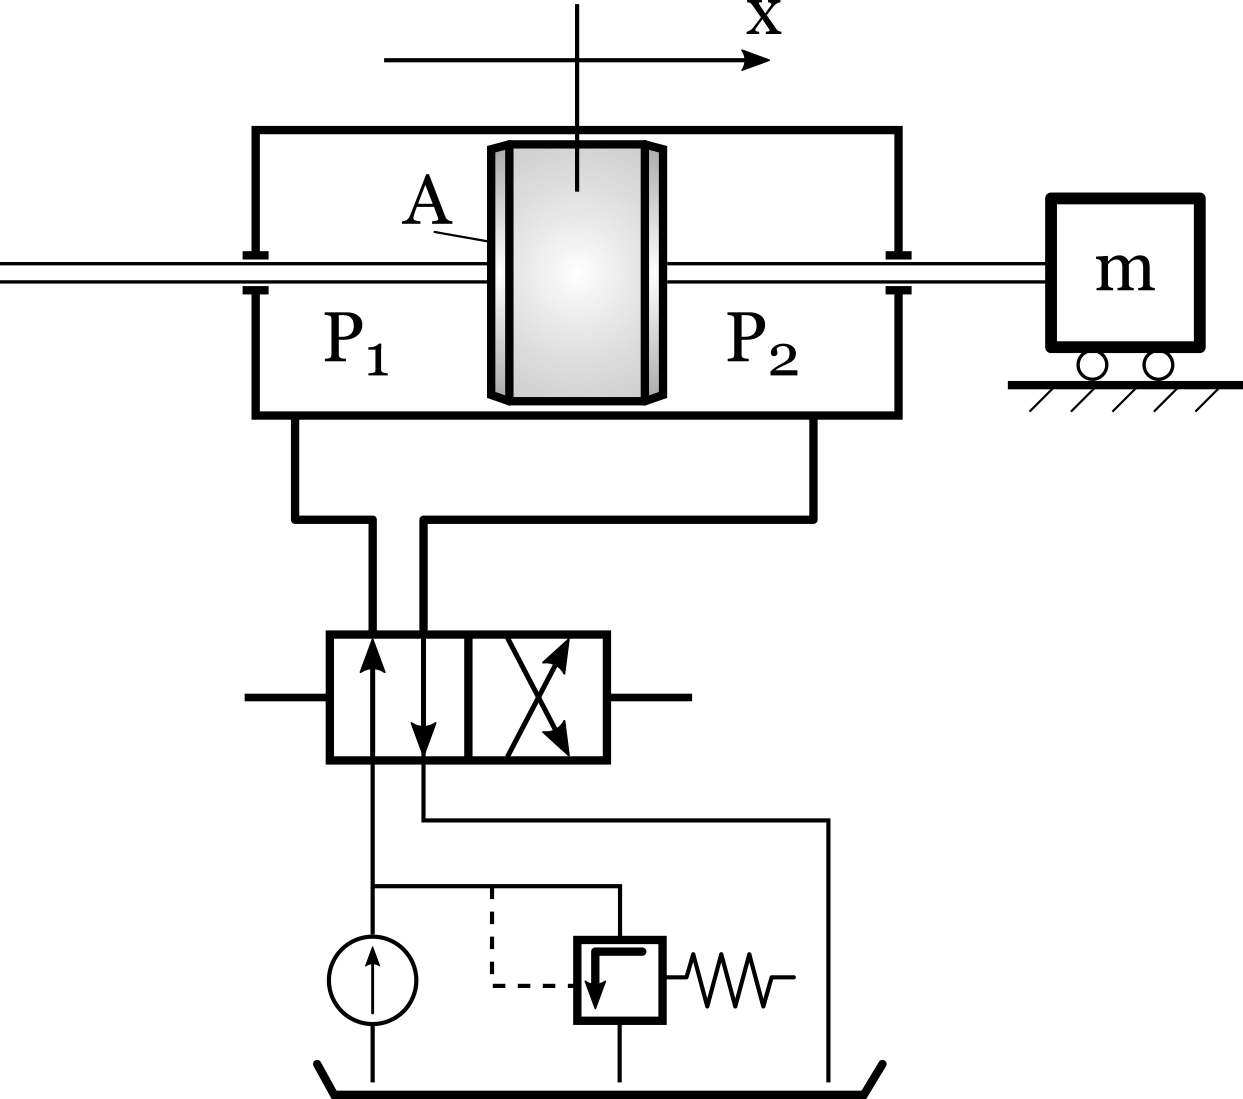
\includegraphics[width=0.5\textwidth]{graphics/munkahenger_fancy.png}
\caption{Munkahenger szabályozása.}
\label{fig:munkahenger}
\end{figure}

A dugattyú mozgását az alábbi másodrendű differenciálegyenlettel írhatjuk le:
%
\begin{equation}
m \ddot{x} + k \dot{x} = A \Delta p, 
\end{equation}
%
\noindent ahol 
%
\begin{equation}
	\Delta p = p_1- p_2 = \left\{
	\begin{matrix}
	+\Delta \tilde{p}, \mathrm{ha} & H(x) > 0\\
	-\Delta \tilde{p}, \mathrm{ha} & H(x) < 0
	\end{matrix}\,.
	\right. 
\end{equation}
%
\indent A szabályozás során a munkahengert az $x_{\rm k} = 0$ pozícióba kívánjuk mozgatni. Ehhez a $H(x)$ függvényt egy PD szabályozási stratégia alapján írjuk elő:
%
\begin{equation} \label{eq:Hx}
H(x) = -P (x - x_{\rm k}) - D \dot{x} = -P x - D \dot{x},
\end{equation}
%
ahol az arányos és differenciáló tagok pozitívak: $P > 0$ és $D > 0$. A dinamikai rendszert az 
%
\begin{equation}
x = (x_1 \; x_2)^{\rm T} = (x \; v)^{\rm T} 
\end{equation}
\noindent változó bevezetésével elsőrendű alakra hozzuk. Ekkor a két vektormező a következő alakú:
%
\begin{equation}
F_1(x) = \left(
\begin{matrix}
x_2\\
\frac{A \Delta \tilde{p}}{m} - \frac{k}{m} x_2
\end{matrix}
\right), \quad
F_2(x) = \left(
\begin{matrix}
x_2\\
-\frac{A \Delta \tilde{p}}{m} - \frac{k}{m} x_2
\end{matrix}
\right). 
\end{equation}
%
\noindent Mivel $\dot{x}=v=x_2$, a $H(x)$ által meghatározott kapcsolóvonal egyenlete a \eqref{eq:Hx}~egyenlet alapján
%
\begin{equation}
\sum = \left\{x: x_2 = -\frac{P}{D} x_1 \right\}\,,
\end{equation}
%
\noindent a kapcsolóvonalra merőleges irányt kijelölő $H_x$ gradiens pedig
%
\begin{equation}
H_x = \left(
\begin{matrix}
-P\\
-D
\end{matrix}\right) \,.
\end{equation}

A kapcsolóvonal $\sum_{\rm s}$ csúszó régiója a
%
\begin{equation}
\langle F_1, H_x \rangle = -P x_2 - \frac{D A \Delta \tilde{p}}{m} + \frac{D k}{m} x_2 < 0 \,,
\end{equation}
%
\noindent valamint az
%
\begin{equation}
\langle F_2, H_x \rangle = -P x_2 + \frac{D A \Delta \tilde{p}}{m} + \frac{D k}{m} x_2 > 0
\end{equation} 
%
\noindent egyenlőtlenségek által adott. Ezekből a csúszó régió:
%
\begin{equation}
\Sigma_{\rm s} = \{x: -x_2^* < x_2 < x_2^* \} \,,
\end{equation}
%
\noindent ahol
%
\begin{equation} \label{eq:x2csillag}
x_2^* = \frac{D A \Delta \tilde{p}}{|D k - P m|} \,.
\end{equation}
%
\noindent A két vektormezőt, a kapcsolófelületet és a csúszó régiót szemlélteti a \ref{fig:csuszomod_szabalyozas}.~ábra.

\begin{figure}[ht]
\centering
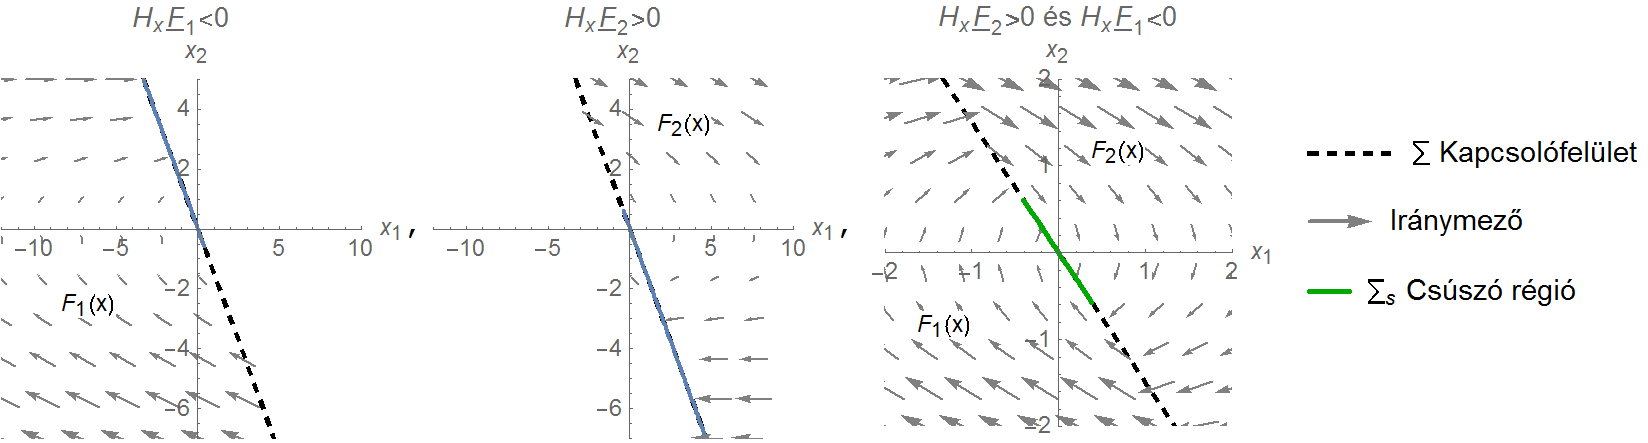
\includegraphics[width=\textwidth]{graphics/sliding_region_PELDA.png}
\caption{Munkahenger csúszómód szabályozása.}
\label{fig:csuszomod_szabalyozas}
\end{figure}

A $\sum_{\rm s}$-en érvényes dinamikát a korábban leírt 
%
\begin{equation}
F_s = F_1 (1-\alpha) + F_2 \alpha 
\end{equation}
%
\noindent vektormező határozza meg, ahol
%
\begin{equation}
\alpha = \frac{\langle F_1, H_x \rangle}{\langle F_1-F_2, H_x \rangle} = \frac{-P x_2 -D \left(\frac{A \Delta \tilde{p}}{m} - \frac{k}{m} x_2\right)}{-D \frac{2A \Delta \tilde{p}}{m}} \,.
%=\frac{D A \Delta \tilde{p} - (D k - P m) x_2}{2 D A \Delta \tilde{p}}
\end{equation}
%
\noindent Ezt $F_s$-be visszahelyettesítve, a kapcsolóvonalra megszorított dinamika
%
\begin{equation}
\begin{split}
F_s & = F_1 (1-\alpha) + F_2 \alpha = F_1 + \alpha (F_2-F_1) =  \\ & =
\begin{pmatrix}
x_2\\
\frac{A \Delta \tilde{p}}{m} - \frac{k}{m} x_2
\end{pmatrix} +
\alpha \begin{pmatrix}
0 \\
-\frac{2A \Delta \tilde{p}}{m}
\end{pmatrix} =
\begin{pmatrix}
x_2 \\
-\frac{P}{D}x_2
\end{pmatrix}
\end{split}
\end{equation}
%
\noindent vagyis
\begin{equation}
\left. \dot{x}_1 \right|_{\Sigma_s} = x_2, \qquad \left. \dot{x}_2 \right|_{\Sigma_s} = -\frac{P}{D} x_2.
\end{equation}
%

\underline{Megjegyzés:} $F_s$ második komponensét a $\sum$ kapcsolóvonal egyenletének idő szerinti deriválásával is meg lehet kapni.

A kapcsolóvonalra megszorított dinamika egy exponenciálisan csillapodó sebességű mozgást ír le, és a rendszer a kapcsolóvonalon tart a $(0 \; 0)^{\rm T}$ egyensúlyi helyzethez.  A $P/D$ hányados növelésével a beállás gyorsasága növelhető, hiszen ekkor a csúszó megoldás egyre gyorsabban tart az origóhoz. Viszont annak érdekében, hogy a sliding mode lehetséges legyen, a \eqref{eq:x2csillag} egyenletben leírt $x_2^*$ kifejezésnek pozitívnak kell lennie, így adódik, hogy 
%
\begin{equation}
\frac{D A \Delta \tilde{p}}{|D k - P m|} >0\,,
\end{equation}
%
\noindent ami akkor teljesül, ha
%
\begin{equation}
\frac{P}{D}m <k\,,
\end{equation}
%
\noindent amiből látszik, hogy a viszkózus csillapítás nem lehet akármekkora. A csúszómód terület csökken, ha $P/D$ nő, akár el is tűnhet.

Szimulációs példát mutat a \ref{fig:sliding_mode_control}.~ábra. A szimuláció során felhasznált paraméterértékeket a \ref{table:parameter}.~táblázat tartalmazza. $x_1(0) = -12$~m és $x_2(0) = 0.2$~m/s kezdeti feltételekkel indítva a szimulációt, a kapcsolófelületen áthaladva, a csúszó felületre kerül a megoldás, majd a rendszer a kapcsolóvonalon tart a $(0 \; 0)^{\rm T}$ egyensúlyi helyzethez.
%
\begin{table}[h!]
	\caption{Paraméterértékek} 
	\vspace{0.1 cm}
	\centering
	\begin{tabular}{|c|c|c|c|c|c|} \hline
	$P$ [1/s] & $D$ [1] & $m$ [kg] & $A$ $[{\rm m}^2]$ & $\Delta \tilde{p}$ [Pa] & $k$ [Ns/m] \\ 	\hline
	$0.3$ & $0.2$ & $0.7$ & $0.5$ & $1$ & $0.1$ \\ \hline
	\end{tabular}
	\label{table:parameter}
\end{table}
%
\begin{figure}[ht]
\centering
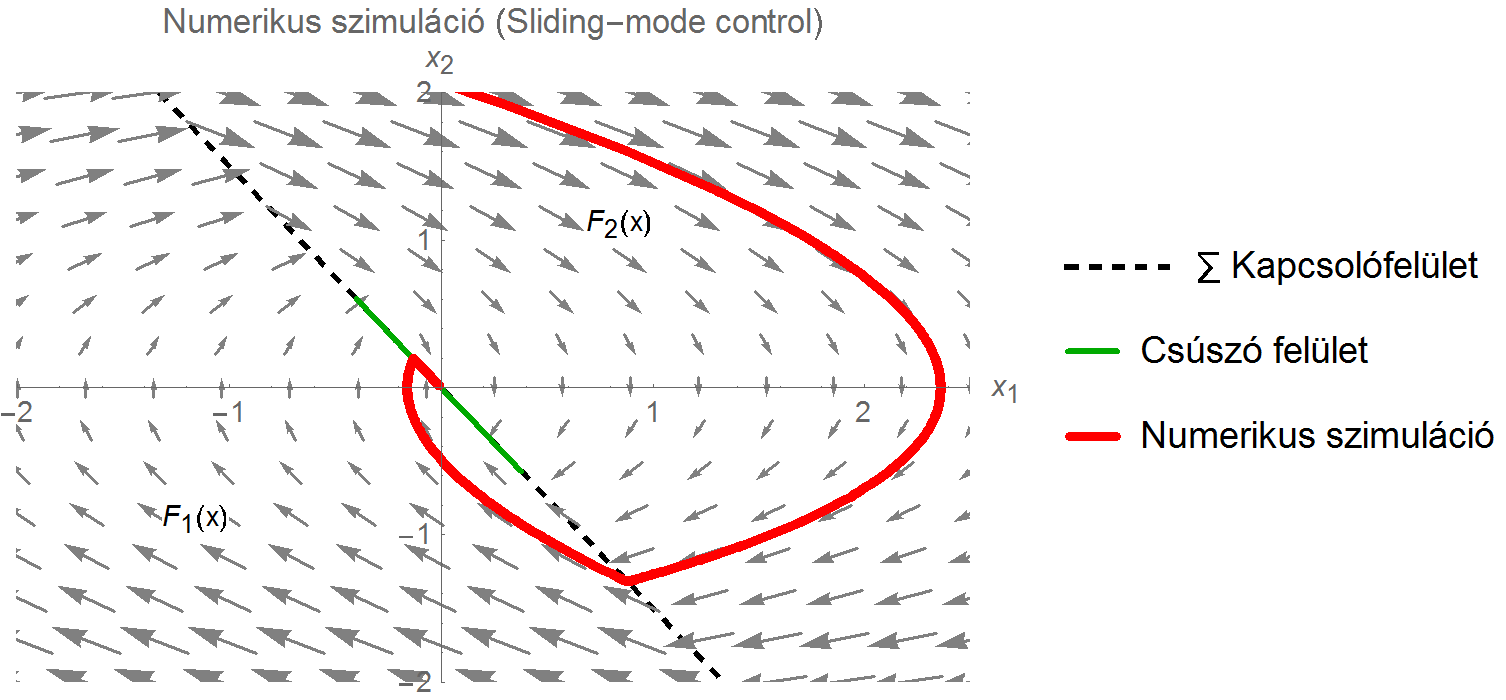
\includegraphics[width=\textwidth]{graphics/sliding_mode_control.png}
\caption{A csúszómód szabályozás által eredményezett trajektória. Kezdeti feltételek: $x_1(0) = -12$~m, $x_2(0) = 0.2$~m/s.}
\label{fig:sliding_mode_control}
\end{figure}

\clearpage